\documentclass{article}
\usepackage[preprint]{neurips_2025}
\usepackage[utf8]{inputenc}
\usepackage[T1]{fontenc}
\usepackage{amsmath,amssymb,booktabs,tabularx,graphicx,xcolor,float,placeins,hyperref}
\hypersetup{colorlinks=true,linkcolor=blue,urlcolor=blue,citecolor=blue}
\makeatletter
\renewcommand{\@noticestring}{COMP6704 --- Member 3 evidence package; not the complete group submission.}
\makeatother
\newcommand{\owner}[1]{\textcolor{blue!55!black}{\textbf{(#1)}}}
\title{RMSProp and Momentum-Free ADOPT:\\Controlled CPU Experiments for COMP6704}
\author{Group Member 3\\Name and student ID: to be supplied before submission}
\begin{document}
\maketitle
\begin{abstract}
We compare independently implemented RMSProp and ADOPT with $\beta_1=0$ on Fashion-MNIST,
CIFAR-10 and Tiny Shakespeare using the shared Member 4 architecture and budget specification.
Validation-only tuning precedes 18 main CPU runs. Under 300 gradient calls, RMSProp performs
better on Fashion and text, while CIFAR results are close. A 240-run unconstrained synthetic
diagnostic shows that previous-moment normalization reduces asymmetric-noise bias at
$\beta_2=.9$, with little gap at $.999$. We report implementation checks, paired seeds,
uncertainty and limitations rather than infer a universal optimizer ranking.
Group repository: \url{https://github.com/ZSH-0103/comp6704-group_project}.
This local Member 3 package has not been published there by this task.
\end{abstract}
\section{Problem and methodology}
We study unconstrained empirical-risk minimization
$\min_{\theta\in\mathbb R^d}N^{-1}\sum_{i=1}^N\ell(h_\theta(x_i),y_i)$.
The research question is whether a normalization change that addresses stochastic bias
also helps at a fixed, small training budget. Sections below are ready-to-merge Member 3
contributions; their numbering in the full group report is 2.4, 3.1--3.2, 4.3 and 5.1.
\subsection{RMSProp and momentum-free ADOPT}\label{sec:method-m3}
\owner{Member 3}
For $g_t=\nabla\ell(\theta_{t-1};\xi_t)$, our non-centered, momentum-free RMSProp uses
\begin{equation}
 v_t=\beta_2v_{t-1}+(1-\beta_2)g_t^{\odot2},\qquad
 \theta_t=\theta_{t-1}-\alpha\frac{g_t}{\sqrt{v_t}+\epsilon},\quad v_0=0.
\end{equation}
The current gradient affects both the numerator and its normalizer. With asymmetric noise,
this dependence can change the expected update direction even when $g_t$ is unbiased
\citep{taniguchi2024adopt}; RMSProp's original motivation is coordinate-wise gradient scaling
\citep{hintonrmsprop}.

We implement the $\beta_1=0$ specialization of ADOPT, denoted ADOPT-0, following the
paper's Section 3.1 and its released implementation \citep{taniguchi2024adopt}.
This is a setting of ADOPT, not a newly named published algorithm.
The first gradient call sets $v_0=g_0^{\odot2}$ without moving $\theta$.
Subsequent calls $t=1,2,\ldots$ use
\begin{equation}\label{eq:m3-adopt}
 u_t=\operatorname{clip}\!\left(\frac{g_t}{\max(\sqrt{v_{t-1}},\epsilon)},-t^{1/4},t^{1/4}\right),\quad
 \theta_t=\theta_{t-1}-\alpha u_t,\quad
 v_t=\beta_2v_{t-1}+(1-\beta_2)g_t^{\odot2}.
\end{equation}
All operations are coordinate-wise. The denominator is determined by the past before drawing
the current sample; clipping is the practical reference-code choice. It can itself introduce
bias, so we also test an unclipped version and a current-moment version with the same
initialization, clipping and $\epsilon$ convention. We set $\beta_2=0.999$ and $\epsilon=10^{-8}$
for both main methods. These differ from official ADOPT defaults ($\beta_2=0.9999$,
$\epsilon=10^{-6}$); neither method uses momentum, weight decay, or a learning-rate schedule.

\paragraph{Theory and cost.}
The ADOPT analysis assumes a lower-bounded differentiable objective, an unbiased stochastic
gradient, Lipschitz-continuous gradient and a uniformly bounded gradient second moment.
Its Theorem 4.1 gives an $O(T^{-1/2})$ bound on
$\min_{t\leq T}(\mathbb E\|\nabla f(\theta_{t-1})\|^{4/3})^{3/2}$ with an appropriate
$\alpha=\Theta(T^{-1/2})$, without a restrictive lower bound on $\beta_2$.
That result is not a guarantee for every step size, the clipped practical variant, or our
ReLU networks. Both implementations require $O(d)$ arithmetic and one $d$-element
second-moment buffer. We omit the redundant first-moment buffer when $\beta_1=0$;
this storage figure describes our specialization, not the full reference optimizer.
Fixed-gradient checks agree with PyTorch RMSProp and pinned official ADOPT at
$10^{-12}$ relative/absolute tolerance in float64; save/load and unchanged training-loop
semantics are also checked.

\paragraph{Unconstrained diagnostic.}
We use $f(\theta)=\log\cosh\theta$ on $\mathbb R$, with optimum $\theta^*=0$, and
$g=\tanh\theta+\xi$, where $\Pr(\xi=-1)=0.9$ and $\Pr(\xi=9)=0.1$.
Then $\mathbb E[g\mid\theta]=f'(\theta)$, $\operatorname{Var}(g\mid\theta)=9$,
$\mathbb E[g^2\mid\theta]\leq10$, and $f$ is 1-smooth and lower-bounded.
This avoids importing the paper's constrained toy problem into an unconstrained study.
We fix $\theta_0=2$, $\alpha=0.01$, 10,000 gradient calls, $\beta_2\in\{0.9,0.99,0.999\}$,
and 20 paired noise seeds (101--120). The primary diagnostic metric is mean objective gap
over the last 1,000 calls. It tests finite-budget behavior, not an asymptotic rate.

\section{Experimental setup}
\subsection{Datasets and preprocessing}
\owner{Member 3; specification aligned with the supplied Member 4 code.}
We use Fashion-MNIST \citep{xiao2017fashion}, CIFAR-10 \citep{krizhevsky2009}, and
Tiny Shakespeare \citep{karpathychar}. For each image task, a permutation with split seed
6704 selects training examples, followed by a disjoint validation subset from the official
training data. A separate permutation from the same generator selects the official-test
subset. These are random subsets, not stratified samples. Full indices and SHA-256 split
fingerprints are saved in \texttt{data/manifests/}. Fashion inputs use mean/std
$0.2860/0.3530$; CIFAR channels use means $(0.4914,0.4822,0.4465)$ and standard deviations
$(0.2470,0.2435,0.2616)$. There is no augmentation.

Text boundaries are character offsets 892,312 and 1,003,851. Each contiguous split is
windowed separately into 64-character inputs and one-character-shifted targets, so windows
cannot cross boundaries. The sorted vocabulary is obtained from the entire source text,
as in Member 4's code; this uses held-out character inventory but no held-out loss for fitting.
This choice and overlapping evaluation windows limit the interpretation of generalization.

\begin{table}[H]\centering\small
\caption{Actual common task specification (Member 3). Text sizes count possible windows.}
\label{tab:data}
\begin{tabularx}{\linewidth}{lXrr}\toprule
Task (writer) & Model & Train / validation / test & Parameters\\\midrule
Fashion (M3) & ReLU MLP $784\to128\to64\to10$ & 6,000 / 1,000 / 1,000 & 109,386\\
CIFAR (M3) & Two-convolution CNN & 5,000 / 1,000 / 1,000 & 25,578\\
Text (M3) & Character GRU & 892,248 / 111,475 / 111,479 & 25,121\\
\bottomrule\end{tabularx}\end{table}

\subsection{Model definitions and executed protocol}
\owner{Member 3; exact counts are checked against the generated dataset summary.}
The CNN uses $3\times3$ convolutions with padding 1, channels $3\to16\to32$,
ReLU and $2\times2$ max pooling after each convolution, and a $32\cdot8\cdot8\to10$ classifier.
The GRU has a 65-character vocabulary, embedding dimension 32, one hidden layer of width 64,
and a 64-to-65 output projection. All parameters are unconstrained; loss is cross-entropy
(CE), averaged over images or target characters. No model uses dropout or batch normalization.

Main training uses 300 gradient calls, batches of 64 images or 32 text windows, and seeds
1, 2, 3. Batches are sampled with replacement using seed $100000+\text{training seed}$.
Within each task/seed pair, initialization and sampled batch indices match exactly, as
verified by hashes. ADOPT-0 makes 299 parameter updates because its first call initializes
$v$. Validation-only tuning uses seed 11, 100 calls per trial and
$\alpha\in\{0.0003,0.001,0.003\}$ for each optimizer/task. The minimum final validation CE
selects the learning rate before any main test evaluation.

Evaluation occurs at calls 0, 50, \ldots, 300, using the first 1,024 examples of each split
(all 1,000 examples for image validation/test). For text these are overlapping windows,
covering only a short prefix of each held-out region. Training CE also uses this fixed prefix,
not all training examples. Each final model is tested once. Times include training and scheduled
train/validation evaluation, but exclude downloads, preprocessing and final test evaluation;
the logs additionally retain total time including the test. All runs use an Apple M1 Pro,
16 GiB RAM, CPU only, four PyTorch threads, Python 3.12.14 and PyTorch 2.14.1.
These are aligned settings, not proof of identical Member 4 runs: that member's actual
manifests, framework version and evaluation-call overrides were not supplied.

\section{Results}
\subsection{RMSProp versus momentum-free ADOPT}\label{sec:results-m3}
\owner{Member 3; all entries and analysis in this subsection.}
We test whether excluding the current gradient from its normalizer reduces bias under
asymmetric noise, and whether that benefit also appears in short neural-network training.
All 18 main runs and 240 diagnostic runs completed without nonfinite values.

\begin{table}[H]\centering\small
\caption{M3-MAIN (Member 3): mean $\pm$ sample SD over three seeds, all $3/3$ completed.
Test quality is accuracy (\%) for images and CE (nats/character) for text; train/validation
columns are CE. Time includes training and scheduled evaluation, excluding final test.}
\label{tab:m3-main}
\begin{tabular}{llrrrr}\toprule
Task & Method (M3) & Train CE & Val CE & Test quality & Time (s)\\\midrule
Fashion & RMSProp & $.368\pm.019$ & $.439\pm.020$ & $81.17\pm.29$ & $2.04\pm.02$\\
 & ADOPT-0 & $.400\pm.053$ & $.481\pm.047$ & $79.43\pm.91$ & $2.06\pm.01$\\
CIFAR & RMSProp & $1.224\pm.057$ & $1.409\pm.060$ & $47.47\pm2.18$ & $9.49\pm.07$\\
 & ADOPT-0 & $1.183\pm.092$ & $1.425\pm.091$ & $47.33\pm2.45$ & $9.59\pm.16$\\
Text & RMSProp & $1.931\pm.014$ & $1.809\pm.008$ & $2.028\pm.012$ & $4.66\pm.02$\\
 & ADOPT-0 & $2.097\pm.016$ & $1.961\pm.021$ & $2.086\pm.013$ & $4.71\pm.04$\\
\bottomrule\end{tabular}\end{table}

RMSProp attains higher Fashion test accuracy by a paired $1.73\pm0.76$ percentage points
and lower text test CE by $0.058\pm0.016$ nats/character. CIFAR test accuracy differs by only
$0.13\pm0.65$ points in favor of RMSProp; three seeds do not establish a general ranking.
ADOPT-0 obtains lower CIFAR training CE without better held-out quality.
Selected learning rates are $0.0003/0.001$ (RMSProp/ADOPT-0) on both image tasks and
$0.003/0.003$ on text. Text optima lie at the search-grid boundary; image RMSProp selects
the lower boundary. Our equal three-trial, 100-call search is limited, and may favor
hyperparameters suited to early progress over performance at 300 calls.

\begin{table}[H]\centering\small
\caption{M3-DIAG (Member 3): last-1,000-call mean objective gap, then mean $\pm$ sample SD
over 20 seeds per cell. All $20/20$ runs per cell completed; 10,000 calls, $\alpha=0.01$.}
\label{tab:m3-diag}
\begin{tabular}{lrrr}\toprule
Method / control (M3) & $\beta_2=.9$ & $\beta_2=.99$ & $\beta_2=.999$\\\midrule
RMSProp & $.1094\pm.0718$ & $.0094\pm.0094$ & $.0084\pm.0069$\\
ADOPT-0 & $.0135\pm.0198$ & $.0084\pm.0072$ & $.0084\pm.0068$\\
Current moment, matched clip & $.1094\pm.0718$ & $.0094\pm.0094$ & $.0084\pm.0069$\\
ADOPT-0, no clip & $.0112\pm.0118$ & $.0084\pm.0072$ & $.0084\pm.0068$\\
\bottomrule\end{tabular}\end{table}

At $\beta_2=.9$, RMSProp's tail-average parameter is $0.448$, versus $-0.008$ for ADOPT-0;
the optimum is zero. The matched current-moment control retains RMSProp-like bias,
supporting the role of normalization timing beyond initialization and clipping.
At $\beta_2=.999$, objective gaps are nearly equal, consistent with weaker current-sample
influence on a slowly changing denominator. This finite-budget observation does not prove
nonconvergence or verify a convergence rate.

\begin{figure}[H]\centering
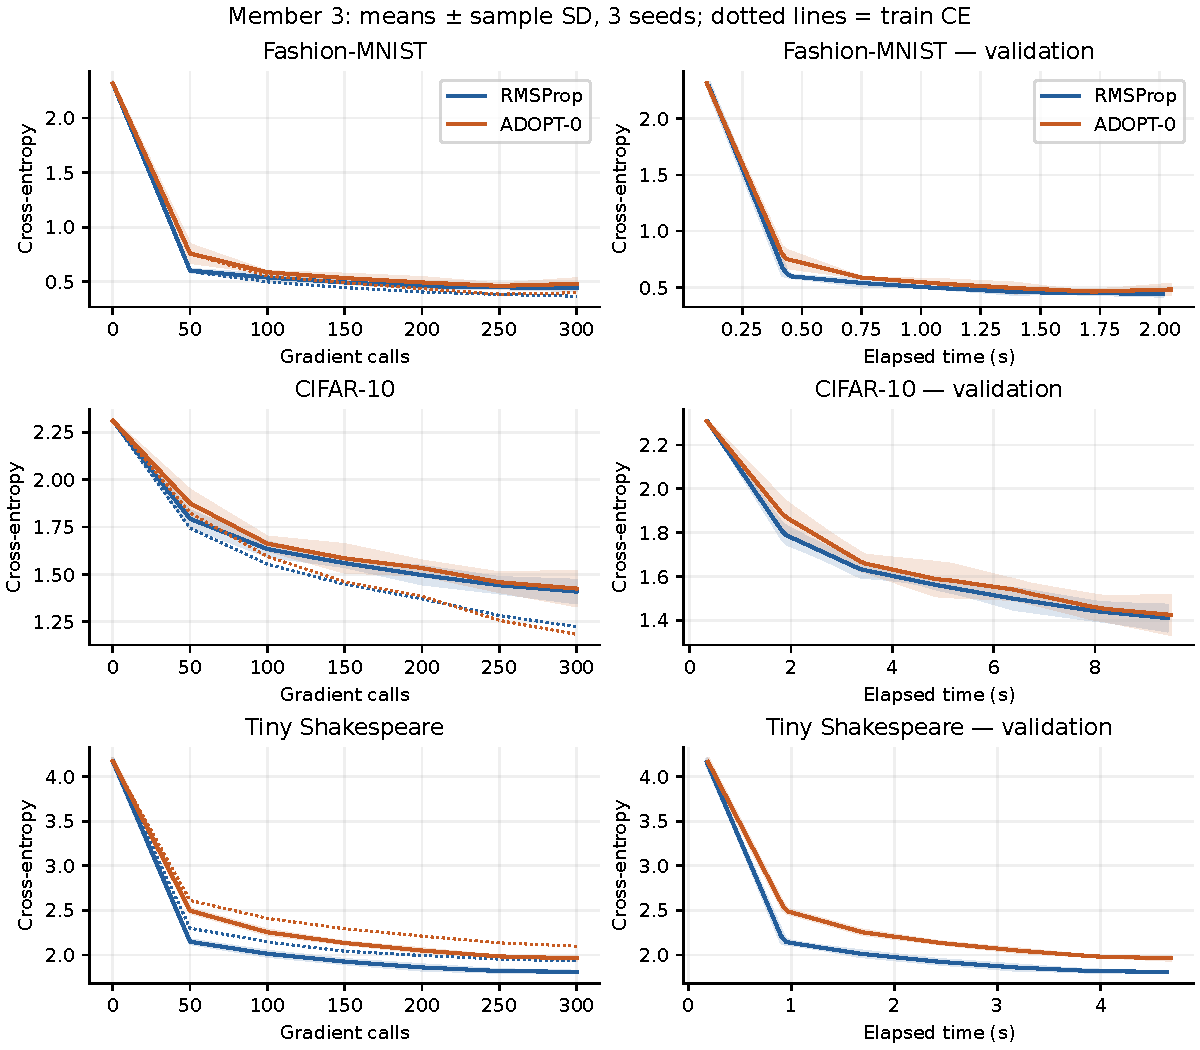
\includegraphics[width=.94\linewidth]{figures/member3_overview.pdf}
\caption{Member 3: solid curves show validation CE, dotted curves show mean training CE;
bands are $\pm1$ sample SD across three seeds. Left: gradient calls. Right: validation CE
interpolated onto a common time grid within each optimizer's observed interval.
Evaluation uses the fixed prefixes described in Setup.}\label{fig:m3-overview}
\end{figure}

\paragraph{Stability and cost.}
Both methods first pass the predeclared validation thresholds (1.0/2.0/3.0) at call 50
in every seed. This coarse metric cannot distinguish their early progress.
ADOPT-0 is approximately 1.0--1.1\% slower here; such small single-machine timing differences
are not a robust efficiency ranking. Both store 437,544 / 102,312 / 100,484 bytes of optimizer
state tensors on Fashion / CIFAR / Text. There are no observed failures, but only three main
seeds and 300 calls; this does not establish general numerical stability.
\FloatBarrier

\section{Discussion}
\subsection{When do the modifications help?}
\owner{Member 3; this paragraph integrates the available Member 3 evidence.}
Tables~\ref{tab:m3-main} and~\ref{tab:m3-diag} distinguish a mechanism benefit from a
practical win. Using a previous second moment reduces the bias observed in the asymmetric-noise
diagnostic at $\beta_2=.9$, including against a control with matched clipping. At the main
setting $\beta_2=.999$, the diagnostic gap is small and ADOPT-0 does not improve held-out
quality on any tested task. Initialization, clipping and transient dynamics provide alternative
explanations for the short-training results; the neural experiments do not isolate these factors.
There is no reduction in tuning effort: both methods receive the same three trials per task.

These conclusions apply to the tested momentum-free specialization, small models, narrow
learning-rate grid and short budget. Image subsets are small; text evaluation covers overlapping
prefix windows; only three main seeds are used. The full paper's default ADOPT, larger models,
longer horizons and complete held-out text regions could behave differently. Results from
Members 1, 2 and 4 must be added before drawing a conclusion across all eight optimizers;
Member 4 supplied configuration and shared code, not measured results for that comparison.

\paragraph{Reproduction.}
See the package README, frozen configurations, data manifests, per-run logs and
\texttt{scripts/export\_results.py}. All reported table entries are generated from measured
logs and rounded only for display; mean $\pm$ SD denotes sample standard deviation, not a
confidence interval. The package includes a hash-verified ZIP and the four editable section files.
\begin{figure}[H]\centering
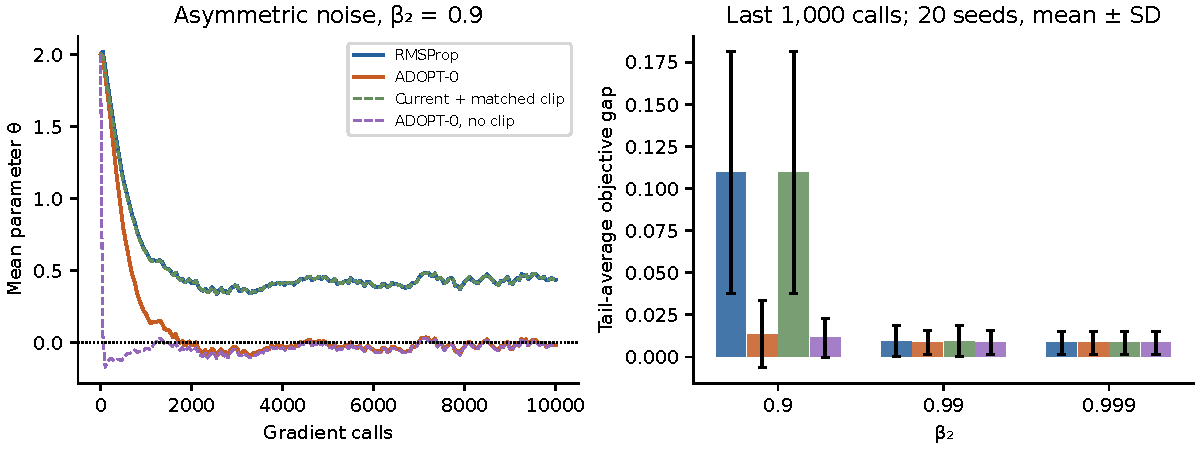
\includegraphics[width=\linewidth]{figures/member3_diagnostic.pdf}
\caption{Additional Member 3 mechanism view. Left: mean parameter trajectory over 20 seeds at
$\beta_2=.9$; zero is optimal. Right: tail-average objective gap and sample SD over 20 seeds.
The current-moment control retains the ADOPT initialization, epsilon convention and clipping.}
\end{figure}
\bibliographystyle{plainnat}
\bibliography{references}
\end{document}
